% ------------------------------------------------------------------------------
% TYPO3 Version 9.1 - What's New - Chapter "Introduction" (Dutch Version)
%
% @author	Michael Schams <schams.net>
% @license	Creative Commons BY-NC-SA 3.0
% @link		http://typo3.org/download/release-notes/whats-new/
% @language	English
% ------------------------------------------------------------------------------
% LTXE-CHAPTER-UID:		7fdf26cc-362160ab-d6c8b905-19722b20
% LTXE-CHAPTER-NAME:	Introduction
% ------------------------------------------------------------------------------

\section{Inleiding}
\begin{frame}[fragile]
	\frametitle{Inleiding}

	\begin{center}\huge{Inleiding}\end{center}
	\begin{center}\huge{\color{typo3darkgrey}\textbf{De feiten}}\end{center}

\end{frame}

% ------------------------------------------------------------------------------
% LTXE-SLIDE-START
% LTXE-SLIDE-UID:		46b65669-bda10096-0377d35a-af3512bf
% LTXE-SLIDE-ORIGIN:	db9ce9bf-51fe8c3b-c6a2649f-aa7018b5 English
% LTXE-SLIDE-TITLE:		TYPO3 Version 9.1 - The Facts
% ------------------------------------------------------------------------------
\begin{frame}[fragile]
	\frametitle{Inleiding}
	\framesubtitle{TYPO3 Versie 9.1 - De feiten}

	\begin{itemize}
		\item Publicatiedatum: 30 januari 2018
		\item Publicatietype: Sprintrelease
	\end{itemize}

	\begin{figure}
		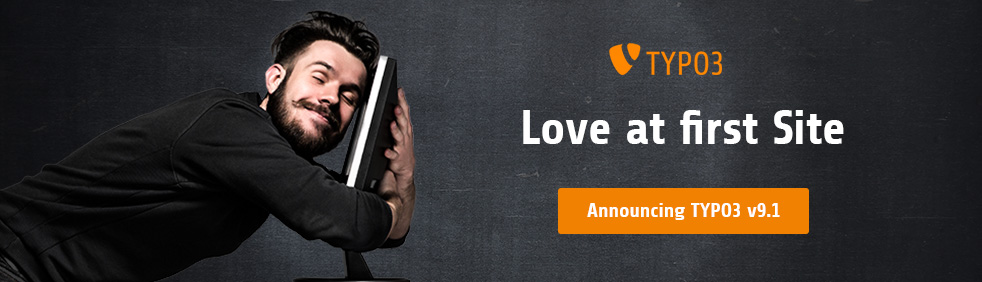
\includegraphics[width=0.95\linewidth]{Introduction/typo3-v91-banner.jpg}
	\end{figure}

\end{frame}

% ------------------------------------------------------------------------------
% LTXE-SLIDE-START
% LTXE-SLIDE-UID:		aad1ecbe-275c8e75-eb4b156e-f6ec29d6
% LTXE-SLIDE-ORIGIN:	baf0e8fa-b8335fbe-911020ab-489d6156 English
% LTXE-SLIDE-TITLE:		System Requirements
% ------------------------------------------------------------------------------
\begin{frame}[fragile]
	\frametitle{Inleiding}
	\framesubtitle{Systeemeisen}

	\begin{itemize}
		\item PHP versie 7.2\newline
			\smaller
				(zal mogelijk worden verlaagd naar PHP 7.1 of 7.0 in een volgende versie)
			\normalsize

		\item PHP instellingen:

			\begin{itemize}
				\item \texttt{memory\_limit} >= 128M
				\item \texttt{max\_execution\_time} >= 240s
				\item \texttt{max\_input\_vars} >= 1500
				\item compilatieoptie \texttt{-}\texttt{-disable-ipv6} moet \underline{niet} worden gebruikt
			\end{itemize}

		\item De meeste databaseservers die worden ondersteund door \textbf{Doctrine DBAL} werken ook met TYPO3.
			De geteste database systemen zijn:
	\end{itemize}

	\begin{figure}
		
\includegraphics[width=0.70\linewidth]{Introduction/logo-databases.png}
	\end{figure}

\end{frame}

% ------------------------------------------------------------------------------
% LTXE-SLIDE-START
% LTXE-SLIDE-UID:		1e044b3c-763e9493-7ef683b2-7a5ac800
% LTXE-SLIDE-ORIGIN:	dfe5c3a8-72a55162-da879770-778ebfec English
% LTXE-SLIDE-TITLE:		Development, Release and Maintenance Timeline
% ------------------------------------------------------------------------------
\begin{frame}[fragile]
	\frametitle{Inleiding}
	\framesubtitle{Ontwikkeling-, versie- en onderhouds-tijdlijn}

	\textbf{TYPO3 v9}

	\begin{figure}
		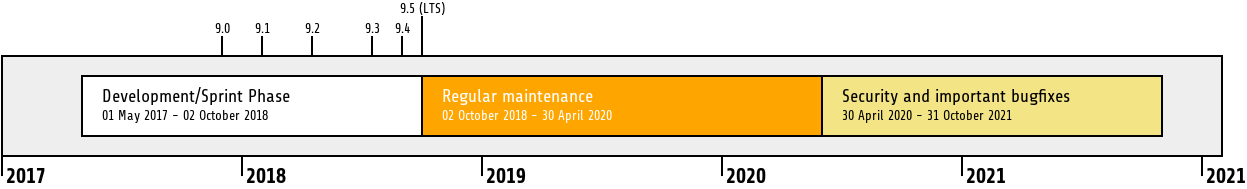
\includegraphics[width=1\linewidth]{Introduction/typo3-v9-lifecycle.png}
	\end{figure}

	\textbf{Verlengde ondersteuning}\newline
	\smaller
		De \href{https://typo3.com}{TYPO3 GmbH} biedt nog 2 jaar extra ondersteuning aan
		voor TYPO3 v9 LTS, zelfs na 31 oktober 2021.
	\normalsize

%	\url{https://typo3.com/our-services/extended-support/}

\end{frame}

% ------------------------------------------------------------------------------
% LTXE-SLIDE-START
% LTXE-SLIDE-UID:		42c41844-5a2bbd69-04e6d5a3-cb748997
% LTXE-SLIDE-ORIGIN:	1c2b096f-e4e0a65c-b0b0d84b-e18889a1 English
% LTXE-SLIDE-TITLE:		TYPO3 v9 Roadmap
% ------------------------------------------------------------------------------
\begin{frame}[fragile]
	\frametitle{Introduction}
	\framesubtitle{TYPO3 v9 Roadmap}

	Verwachte verschijningsdata en de focus van de versie:

	\begin{itemize}

		\item v9.0 \tabto{1.1cm}12/Dec/2017\tabto{3.4cm}Install Tool en paginaboom herschreven,\newline
			\tabto{3.4cm}Vertalen pagina's verbeterd
		\item
			\begingroup
				\color{typo3orange}
					v9.1 \tabto{1.1cm}30/Jan/2018\tabto{3.4cm}Redirect afhandeling
			\endgroup
		\item v9.2 \tabto{1.1cm}10/Apr/2018\tabto{3.4cm}Site configuratie
		\item v9.3 \tabto{1.1cm}12/Jun/2018\tabto{3.4cm}Leesbare URL's
		\item v9.4 \tabto{1.1cm}04/Sep/2018\tabto{3.4cm}Content bewerken in de frontend
		\item v9.5 \tabto{1.1cm}02/Oct/2018\tabto{3.4cm}LTS versie

	\end{itemize}

	\smaller
		\url{https://typo3.org/news/article/typo3-v9-roadmap/}
	\normalsize

\end{frame}

% ------------------------------------------------------------------------------
% LTXE-SLIDE-START
% LTXE-SLIDE-UID:		7a7efe2d-82f4fa56-ab1acdc0-c6c8dccd
% LTXE-SLIDE-ORIGIN:	27b13d1c-5c952e3e-d4422d93-0a8a273d English
% LTXE-SLIDE-TITLE:		Installation
% ------------------------------------------------------------------------------
\begin{frame}[fragile]
	\frametitle{Inleiding}
	\framesubtitle{Installatie}

	\begin{itemize}
		\item Officiële \textit{klassieke} installatieprocedure op Linux/Mac OS X\newline
			(DocumentRoot bijvoorbeeld \texttt{/var/www/site/htdocs}):
		\begin{lstlisting}
			$ cd /var/www/site
			$ wget --content-disposition get.typo3.org/9.1
			$ tar xzf typo3_src-9.1.0.tar.gz
			$ cd htdocs
			$ ln -s ../typo3_src-9.1.0 typo3_src
			$ ln -s typo3_src/index.php
			$ ln -s typo3_src/typo3
			$ touch FIRST_INSTALL
		\end{lstlisting}

		\item Symbolische koppelingen op Microsoft Windows:

			\begin{itemize}
				\item Gebruik \texttt{junction} op Windows XP/2000
                				\item Gebruik \texttt{mklink} op Windows Vista en Windows 7
			\end{itemize}

	\end{itemize}
\end{frame}

% ------------------------------------------------------------------------------
% LTXE-SLIDE-START
% LTXE-SLIDE-UID:		bbeb3c4a-d613625f-1847c4c9-156bf2bb
% LTXE-SLIDE-ORIGIN:	2991c08b-8831f59c-56bc188c-e05b8e92 English
% LTXE-SLIDE-TITLE:		Installation using composer
% ------------------------------------------------------------------------------
\begin{frame}[fragile]
	\frametitle{Installatie en Upgrade}
	\framesubtitle{Installatie met \texttt{composer}}

	\begin{itemize}
		\item Installatie met \textit{composer} op Linux/Mac OS X

			\begin{lstlisting}
				$ cd /var/www/site/
				$ composer create-project typo3/minimal
			\end{lstlisting}

		\item Of anders kan een maatwerk \texttt{composer.json} bestand gemaakt worden en dan:

			\begin{lstlisting}
				$ composer install
			\end{lstlisting}

			Een voorbeeld \texttt{composer.json} is te downloaden van:\newline
			\small
				\href{https://git.typo3.org/TYPO3CMS/Distributions/Base.git/blob/HEAD:/composer.json}{git.typo3.org/TYPO3CMS/Distributions/Base.git/blob/HEAD:/composer.json}
			\normalsize

	\end{itemize}
\end{frame}

% ------------------------------------------------------------------------------
% LTXE-SLIDE-START
% LTXE-SLIDE-UID:		5f940149-b9b98325-846ea077-27d89ef4
% LTXE-SLIDE-ORIGIN:	3bc1e21e-cf2c23c4-b1d641af-8e351b92 English
% LTXE-SLIDE-TITLE:		Upgrade to TYPO3 Version 9
% ------------------------------------------------------------------------------
%\begin{frame}[fragile]
%	\frametitle{Introduction}
%	\framesubtitle{Upgrade to TYPO3 Version 9.x}
%
%	\begin{itemize}
%		\item Upgrades only possible from TYPO3 v8 LTS
%		\item TYPO3 < v8 LTS should be updated to TYPO3 v8 LTS first
%	\end{itemize}
%
%	\begin{itemize}
%
%		\item Upgrade instructions:\newline
%			\smaller\url{https://wiki.typo3.org/Upgrade#Upgrading_to_9.1}\normalsize
%		\item Official TYPO3 guide "TYPO3 Installation and Upgrading":
%			\smaller\url{https://docs.typo3.org/typo3cms/InstallationGuide}\normalsize
%		\item General approach:
%			\begin{itemize}
%				\item Check minimum system requirements \small(PHP, MySQL, etc.)
%				\item Review \textbf{deprecation\_*.log} in old TYPO3 instance
%				\item Update all extensions to the latest version
%				\item Deploy new sources and run Install Tool -> Upgrade Wizard
%				\item Review startup module for backend users (optionally)
%			\end{itemize}
%	\end{itemize}
%
%\end{frame}
%
% ------------------------------------------------------------------------------
